\documentclass[12pt, a4paper]{article}
\usepackage[utf8]{inputenc}
\usepackage[T1]{fontenc}
\usepackage{amsmath}
\usepackage{amssymb}
\usepackage[margin=1in]{geometry}
\usepackage{parskip} % Para separar párrafos con espacio en lugar de indentación
\usepackage{xcolor}     % Necesario para definir los colores
\usepackage{listings}   % El paquete principal para el código
\usepackage{hyperref}
\usepackage{graphicx}
\usepackage{float}

\graphicspath{{imagenes/}}


% --- Configuración del Título ---
\title{Informe: Solución Óptima al Problema de Selección de Intervalos de Máxima Cardinalidad}
\author{Nicolás Paz Reyes, Martín Moloeznik y Luca Bogado}
\date{19 de octubre de 2025}

\begin{document}

\maketitle

\section{Descripción Matemática del Problema}

El problema consiste en, dado un conjunto finito $C$ de $n$ intervalos cerrados sobre la recta real, 
encontrar un subconjunto de $C$ de máxima cardinalidad cuyos intervalos sean disjuntos.

Formalmente:

\begin{itemize}
    \item Un conjunto $C = \{(a_i, b_i) \mid a_i, b_i \in \mathbb{R}, a_i \le b_i\}$.
    
    \item Dos intervalos $I_1 = (a_1, b_1)$ e $I_2 = (a_2, b_2)$ son disjuntos (compatibles) si no se superponen. Asumiendo la convención de intervalos semiabiertos $[a, b)$ (como inferimos en nuestro código, donde \texttt{inicioActual >= finUltimo}), la compatibilidad se define como:
    $b_1 \le a_2$ o $b_2 \le a_1$.
    
    \item Debemos encontrar un subconjunto $C' \subseteq C$ tal que:
    \begin{enumerate}
        \item \textbf{Validez:} $\forall I, J \in C', (I \neq J \implies I \text{ y } J \text{ son disjuntos})$.
        \item \textbf{Optimalidad:} $|C'|$ es máximo. Es decir, para cualquier otro subconjunto $S \subseteq C$ que cumpla la condición de validez, se tiene que $|S| \le |C'|$.
    \end{enumerate}
\end{itemize}

\section{Estrategia Greedy y Solución Propuesta}

Para resolver este problema de optimización, proponemos una estrategia \textit{greedy} 
que toma decisiones localmente óptimas en cada paso, con la expectativa de alcanzar una solución 
globalmente óptima.

\subsection*{La Estrategia: "Elegir el que Termina Antes"}

Nuestra estrategia se basa en la intuición de que, para maximizar el número de intervalos seleccionados, 
debemos liberar el "recurso" (los subintervalos) lo antes posible.
El criterio de selección será siempre el intervalo que se encuentre más a la izquierda, por ende podremos ir 
analizando todas las regiones del espacio en donde potencialmente puedan haber subconjuntos de 
intervalos consecutivos disjuntos posibles.


El algoritmo procede de la siguiente manera:

\begin{enumerate}
    \item \textbf{Ordenar:} Ordenar el conjunto $C$ de $n$ intervalos en orden ascendente, según su \textbf{tiempo de finalización} ($b_i$).
    
    \item \textbf{Seleccionar:} Inicializar la solución $G$ con el primer intervalo de $C$ (aquel con el $b_i$ mínimo global). Sea $g_{\text{$b_{menor}$}}$ este intervalo.
    
    \item \textbf{Iterar y Filtrar:} Recorrer $C_o$ (a partir del intervalo \textit{siguiente} a $g_{\text{b\_menor}}$) 
    hasta encontrar el \textit{primer} intervalo $I = (a, b)$ que sea compatible con 
    $g_{\text{b\_menor}}$ (es decir, $a > b_{\text{menor}}$).
    
    \item \textbf{Volver o terminar:}
    \begin{itemize}
        \item \textbf{Si se encontró} dicho intervalo $I$: Añadir $I$ a $G$, actualizar $g_{\text{$b_{menor}$}} = I$, y \textbf{volver al Paso 3} (continuando la búsqueda desde el intervalo \textit{siguiente} a $I$).
        \item \textbf{Si no quedan intervalos} por revisar (o no se encuentran más intervalos compatibles), \textbf{Terminar}. $G$ es la solución final.
    \end{itemize}
\end{enumerate}

Esta estrategia garantiza que, en cada paso, la elección \textit{greedy} es la que elije la máxima cantidad 
de intervalos disjuntos.

\section{Demostración de Optimalidad}

A continuación, demostramos formalmente que la estrategia \textit{greedy} descripta 
("Elegir el que Termina Antes") produce siempre una solución de cardinalidad máxima.

\textbf{Teorema:} El algoritmo \textit{greedy} (G) encuentra una solución óptima.

\textbf{Definiciones:}
\begin{itemize}
    \item Sea $G = \{g_1, g_2, \dots, g_k\}$ la solución encontrada por nuestro algoritmo 
    \textit{greedy}, con $k$ intervalos. Los intervalos están ordenados por su tiempo de finalización, 
    de modo que $b_{g1} \le b_{g2} \le \dots \le b_{gk}$. (Donde $g_i = (a_{gi}, b_{gi})$).
    \item Sea $O = \{o_1, o_2, \dots, o_m\}$ una solución \textbf{óptima} cualquiera, con $m$ intervalos, 
    también ordenados por su tiempo de finalización ($b_{o1} \le b_{o2} \le \dots \le b_{om}$).
\end{itemize}

\textbf{Objetivo:} Demostrar que $k = m$.

Por la definición de optimalidad, $G$ no puede ser más grande que $O$, por lo tanto, sabemos que $m \ge k$. La prueba se centrará en demostrar que $m=k$.

\subsection{Paso a Paso de la Demostración}

\paragraph{1. Caso Base: Soluciones Idénticas}
Si la solución \textit{greedy} $G$ y la solución óptima $O$ son idénticas, entonces $k = m$ y 
ya hemos demostrado que $G$ es óptima. Para el resto de la demostración,es decir, los demás casos, 
asumimos que $G \neq O$.

\paragraph{2. Encontrar la Primera Diferencia}
Si las soluciones no son idénticas, debe existir un primer intervalo en el que difieren. 
Sea $i$ el primer índice tal que $g_i \neq o_i$.
Esto implica que los intervalos anteriores sí coinciden: $g_1 = o_1, g_2 = o_2, \dots, g_{i-1} = o_{i-1}$.

\paragraph{3. La Propiedad Clave de Greedy}
En el paso $i$, nuestro algoritmo \textit{greedy} eligió el intervalo $g_i$. Lo hizo del conjunto de 
todos los intervalos disponibles que no se superponían con $g_{i-1}$.
El intervalo $o_i$ (de la solución óptima) también pertenece a ese conjunto de candidatos válidos, 
ya que $o_i$ es compatible con $o_{i-1}$, y $o_{i-1} = g_{i-1}$.
Por la propia regla de selección del algoritmo (elegir siempre el que finaliza antes, es decir, el "$b$ menor"), es 
imposible que $o_i$ termine antes que $g_i$. Formalmente:
\[ b_{gi} \le b_{oi} \]
Esta es la propiedad fundamental de nuestra estrategia, que usaremos a continuación.

\paragraph{4. Demostración por Argumento de Intercambio}
Ahora, creemos una nueva solución $O'$ a partir de la óptima $O$, reemplazando $o_i$ por $g_i$:
\[ O' = (O \setminus \{o_i\}) \cup \{g_i\} = \{o_1, \dots, o_{i-1}, g_i, o_{i+1}, \dots, o_m\} \]

\textbf{Verificación de Validez de O':} Debemos demostrar que $O'$ sigue siendo un conjunto de intervalos disjuntos.
    \begin{enumerate}
        \item \textbf{Compatibilidad con anteriores ($j < i$):} $g_i$ es compatible con $g_{i-1}$, y como $g_{i-1} = o_{i-1}$, $g_i$ es compatible con $o_{i-1}$.
        \item \textbf{Compatibilidad con posteriores ($j > i$):} Debemos probar que $g_i$ es compatible con $o_{i+1}$.
        \begin{itemize}
            \item Sabemos que $O$ es válida, por lo que $a_{oi+1}\ge b_{oi}$.
            \item Por nuestra \textbf{Propiedad Clave (Paso 3)}, sabemos que $b_{gi} \le b_{oi}$.
            \item Combinando ambas: $a_{oi+1} \ge b_{oi} \ge b_{gi}$.
            \item Esto demuestra que $g_i$ es compatible con $o_{i+1}$.
        \end{itemize}
    \end{enumerate}
\textbf{Optimalidad de O':} $O'$ es una solución válida y tiene tamaño $m$. Por lo tanto, $O'$ 
también es una solución óptima.

\textit{Conclusión del Intercambio:} Hemos demostrado que si $O$ difiere de $G$, podemos transformarla 
en $G$ paso a paso sin alterar su optimalidad. Esto implica que $|G| = |O|$, es decir, $k = m$.

\paragraph{5. Demostración por Contradicción (El caso k + 1)}
Para solidificar la conclusión $k=m$, demostramos que $m > k$ conduce a una contradicción.

Supongamos para llegar al absurdo, que la solución óptima es estrictamente más grande que la solución greedy: $m > k$.\\

Esto trae como \textbf{consecuencia} que si $m > k$ es válido, debe existir un intervalo $o_{k+1}$ en 
la solución óptima $O$. Como $O$ es válida, $o_{k+1}$ debe ser compatible con $o_k$, es decir, $a_{ok+1} \ge b_{ok}$.\\

\textbf{La Contradicción:} Aplicamos nuestra \textbf{Propiedad Clave (Paso 3)}. 
Esta propiedad se mantiene para todo $i \le k$. Por lo tanto, para $i=k$, tenemos $b_{gk} \le b_{ok}$.\\
Combinando los pasos:   \[ a_{ok+1} \ge b_{ok} \ge b_{gk} \]
Esto implica que $a_{ok+1} \ge b_{gk}$. Esta desigualdad significa que $o_{k+1}$ 
\textbf{era un candidato compatible} con $g_k$ (el último intervalo que el \textit{greedy} seleccionó).\\

Sin embargo, el algoritmo \textit{greedy} se detuvo después de $g_k$. Por definición (Paso 4 de nuestra estrategia), esto solo ocurre cuando no quedan más intervalos compatibles.\\
La existencia de $o_{k+1}$ (un intervalo compatible que el \textit{greedy} no seleccionó) 
\textbf{contradice la condición de finalización del algoritmo}.\\


\section{\textbf{Conclusión Final}} 

La suposición ($m > k$) es falsa. Dado que $m \ge k$ y $m \ngtr k$, la única posibilidad restante es que $m=k$.
Hemos demostrado mediante el argumento de intercambio que la solución greedy es óptima. 
Además, hemos reforzado esta conclusión probando por contradicción que ninguna solución puede ser 
estrictamente más grande. Por lo tanto, la estrategia greedy de elegir el intervalo que finaliza 
primero produce siempre una solución de máxima cardinalidad. \textbf{Es óptima}.

\section{Análisis del Programa y Complejidad}

El algoritmo \textit{greedy} descripto (Pasos 1-4) se implementó en Haskell de la siguiente forma.

\begin{figure}[H]
    \centering
    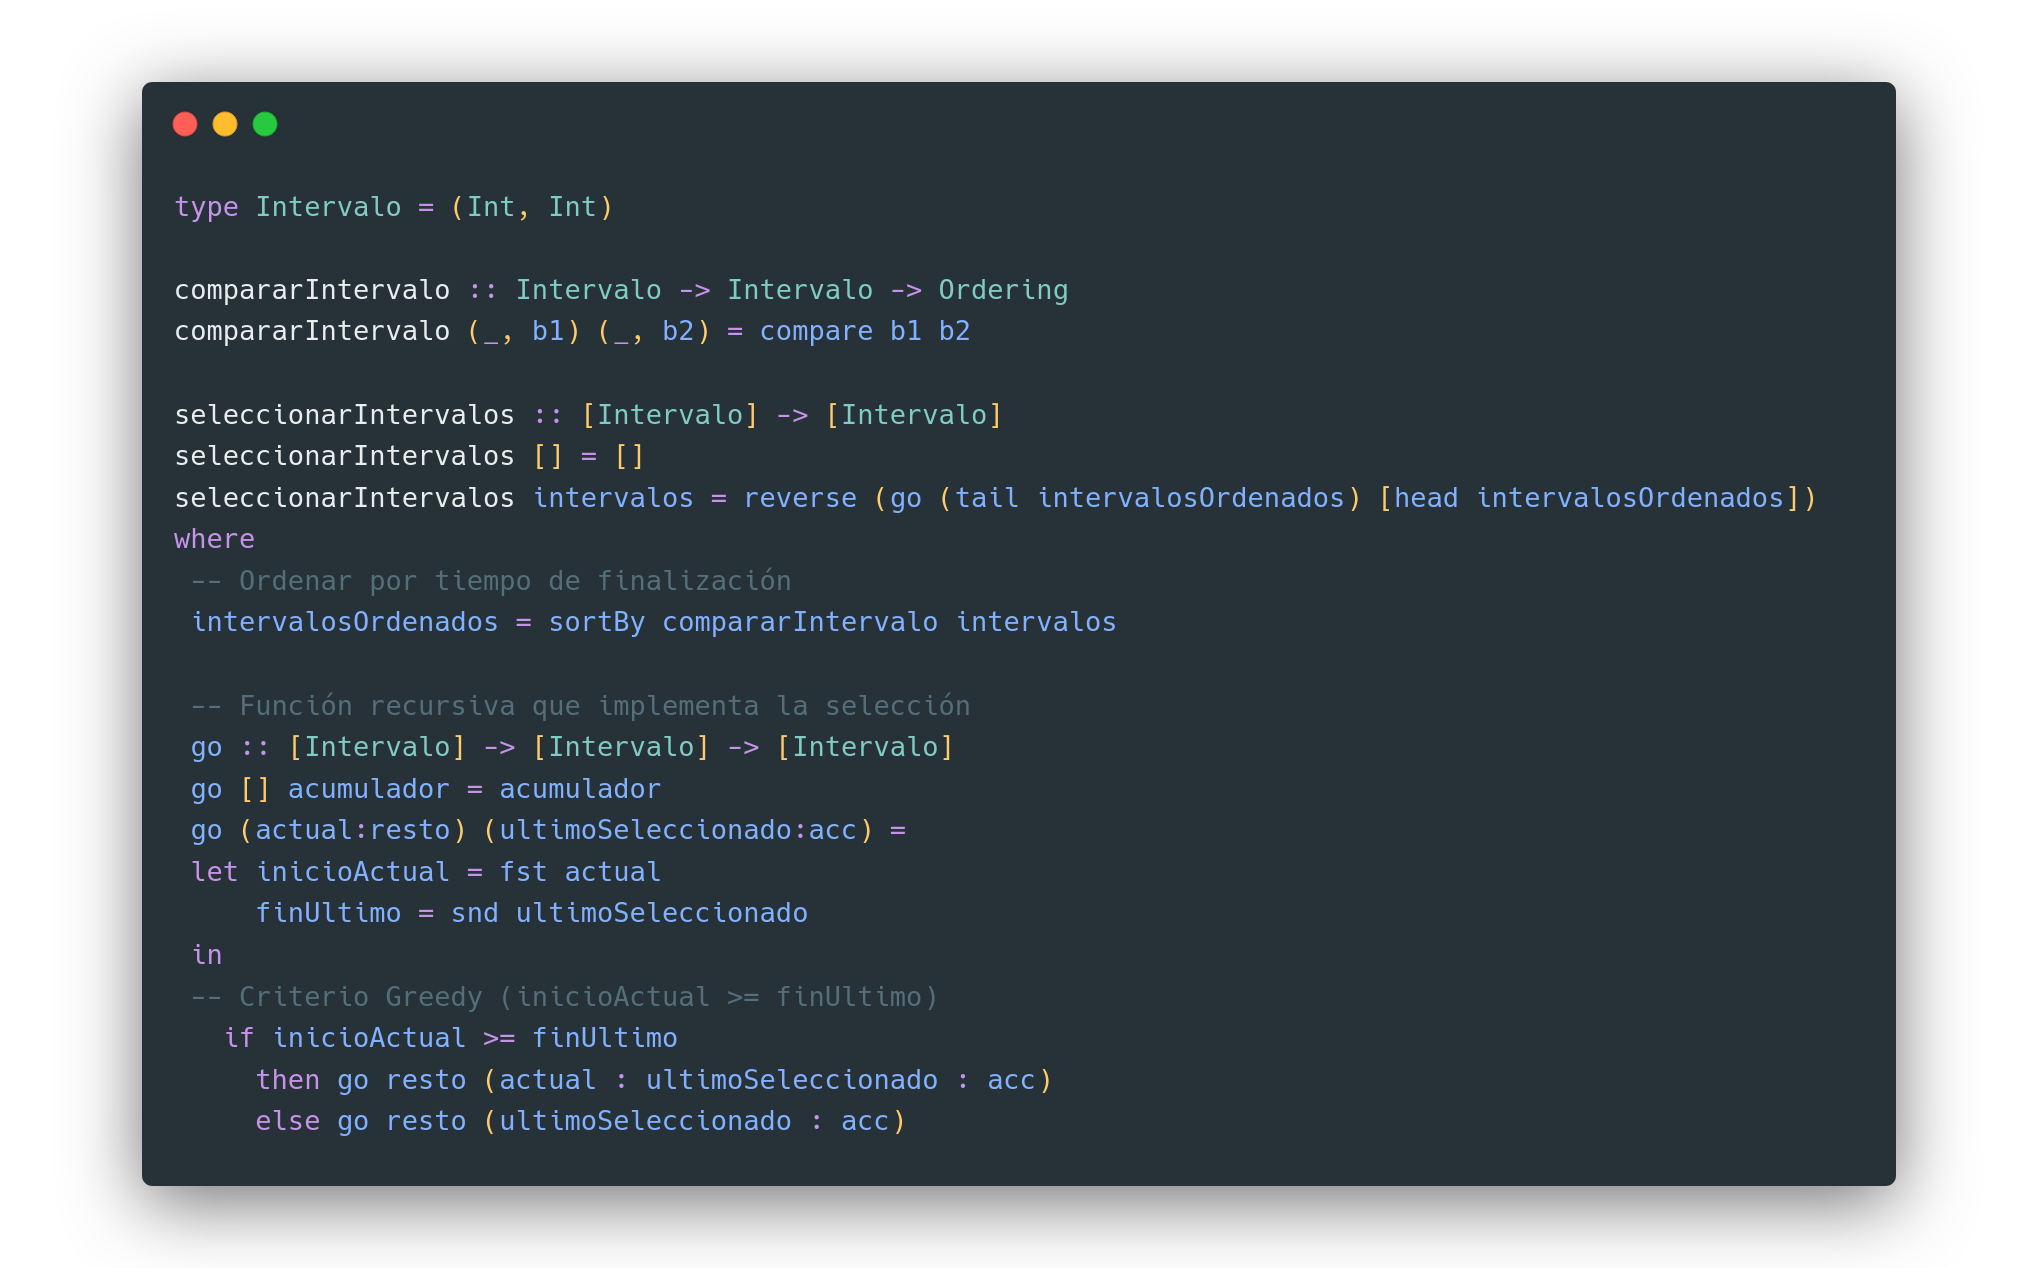
\includegraphics[width=\linewidth]{carbon.png}
    \caption{Nuestra implementación del algoritmo en Haskell.}
    \label{fig:imagencodigo}
\end{figure}


\end{document}